\documentclass[12pt]{article}

\usepackage{fullpage}
\usepackage{graphicx, rotating, booktabs} 
\usepackage{times} 
\usepackage{natbib} 
\usepackage{indentfirst} 
\usepackage{setspace}
\usepackage{grffile} 
\usepackage{hyperref}
\usepackage{adjustbox}
\setcitestyle{aysep{}}


\singlespace
\title{\textbf{Appendix: Alliance Participation, Treaty Depth, and Military Spending}}
%\author{Joshua Alley}
\date{}

\bibliographystyle{apsr}

\begin{document}

\maketitle 

\doublespace 

This online appendix provides more detail about the multilevel model and some checks of the results. 


\section*{Priors}

\autoref{tab:priors} summarizes the prior distributions in the multilevel model. 
All priors are weakly informative relative to the scale of the data. 
$\nu$ is the degrees of freedom for the t-distribution, and the gamma prior is the recommended default prior for STAN. 

\begin{table} % Create a table of priors.
\begin{center}
\begin{tabular}{c} 
$ p(\alpha) \sim N(0, 1)$  \\
$ p(\sigma) \sim \mbox{half-}N(0, 1) $ \\
$ p(\alpha^{yr}) \sim N(0, \sigma^{yr}) $ \\ 
$ p(\sigma^{yr}) \sim N(0, 1) $ \\
$ p(\alpha^{st}) \sim N(0, \sigma^{st}) $ \\ 
$ p(\sigma^{st}) \sim \mbox{half-}N(0, .5) $ \\ 
$ p(\sigma^{all}) \sim \mbox{half-}N(0, .5) $ \\
$ p(\beta) \sim N(0, .5) $ \\
$ p(\gamma) \sim N(0, .5) $ \\ 
$ p(\nu) \sim gamma(2, 0.1)$ 
\end{tabular} 
\caption{Summary of Priors in Multilevel Model} 
\label{tab:priors}
\end{center} 
\end{table} 


\section*{Hamiltonian Monte Carlo Diagnostics}

There were no divergent iterations in either sample running 4 chains for 2,000 iterations with 1,000 warmup iterations. 
The $\hat{R}$ is less than 1.1 for all parameters in both samples. 
Trace plots in \autoref{fig:trace-all-min} indicate good mixing of the chains for the alliance-level parameters. 
Taken together, all of this implies that the chains adequately explored the posterior distribution. 

\begin{figure}[htbp]
	\centering
		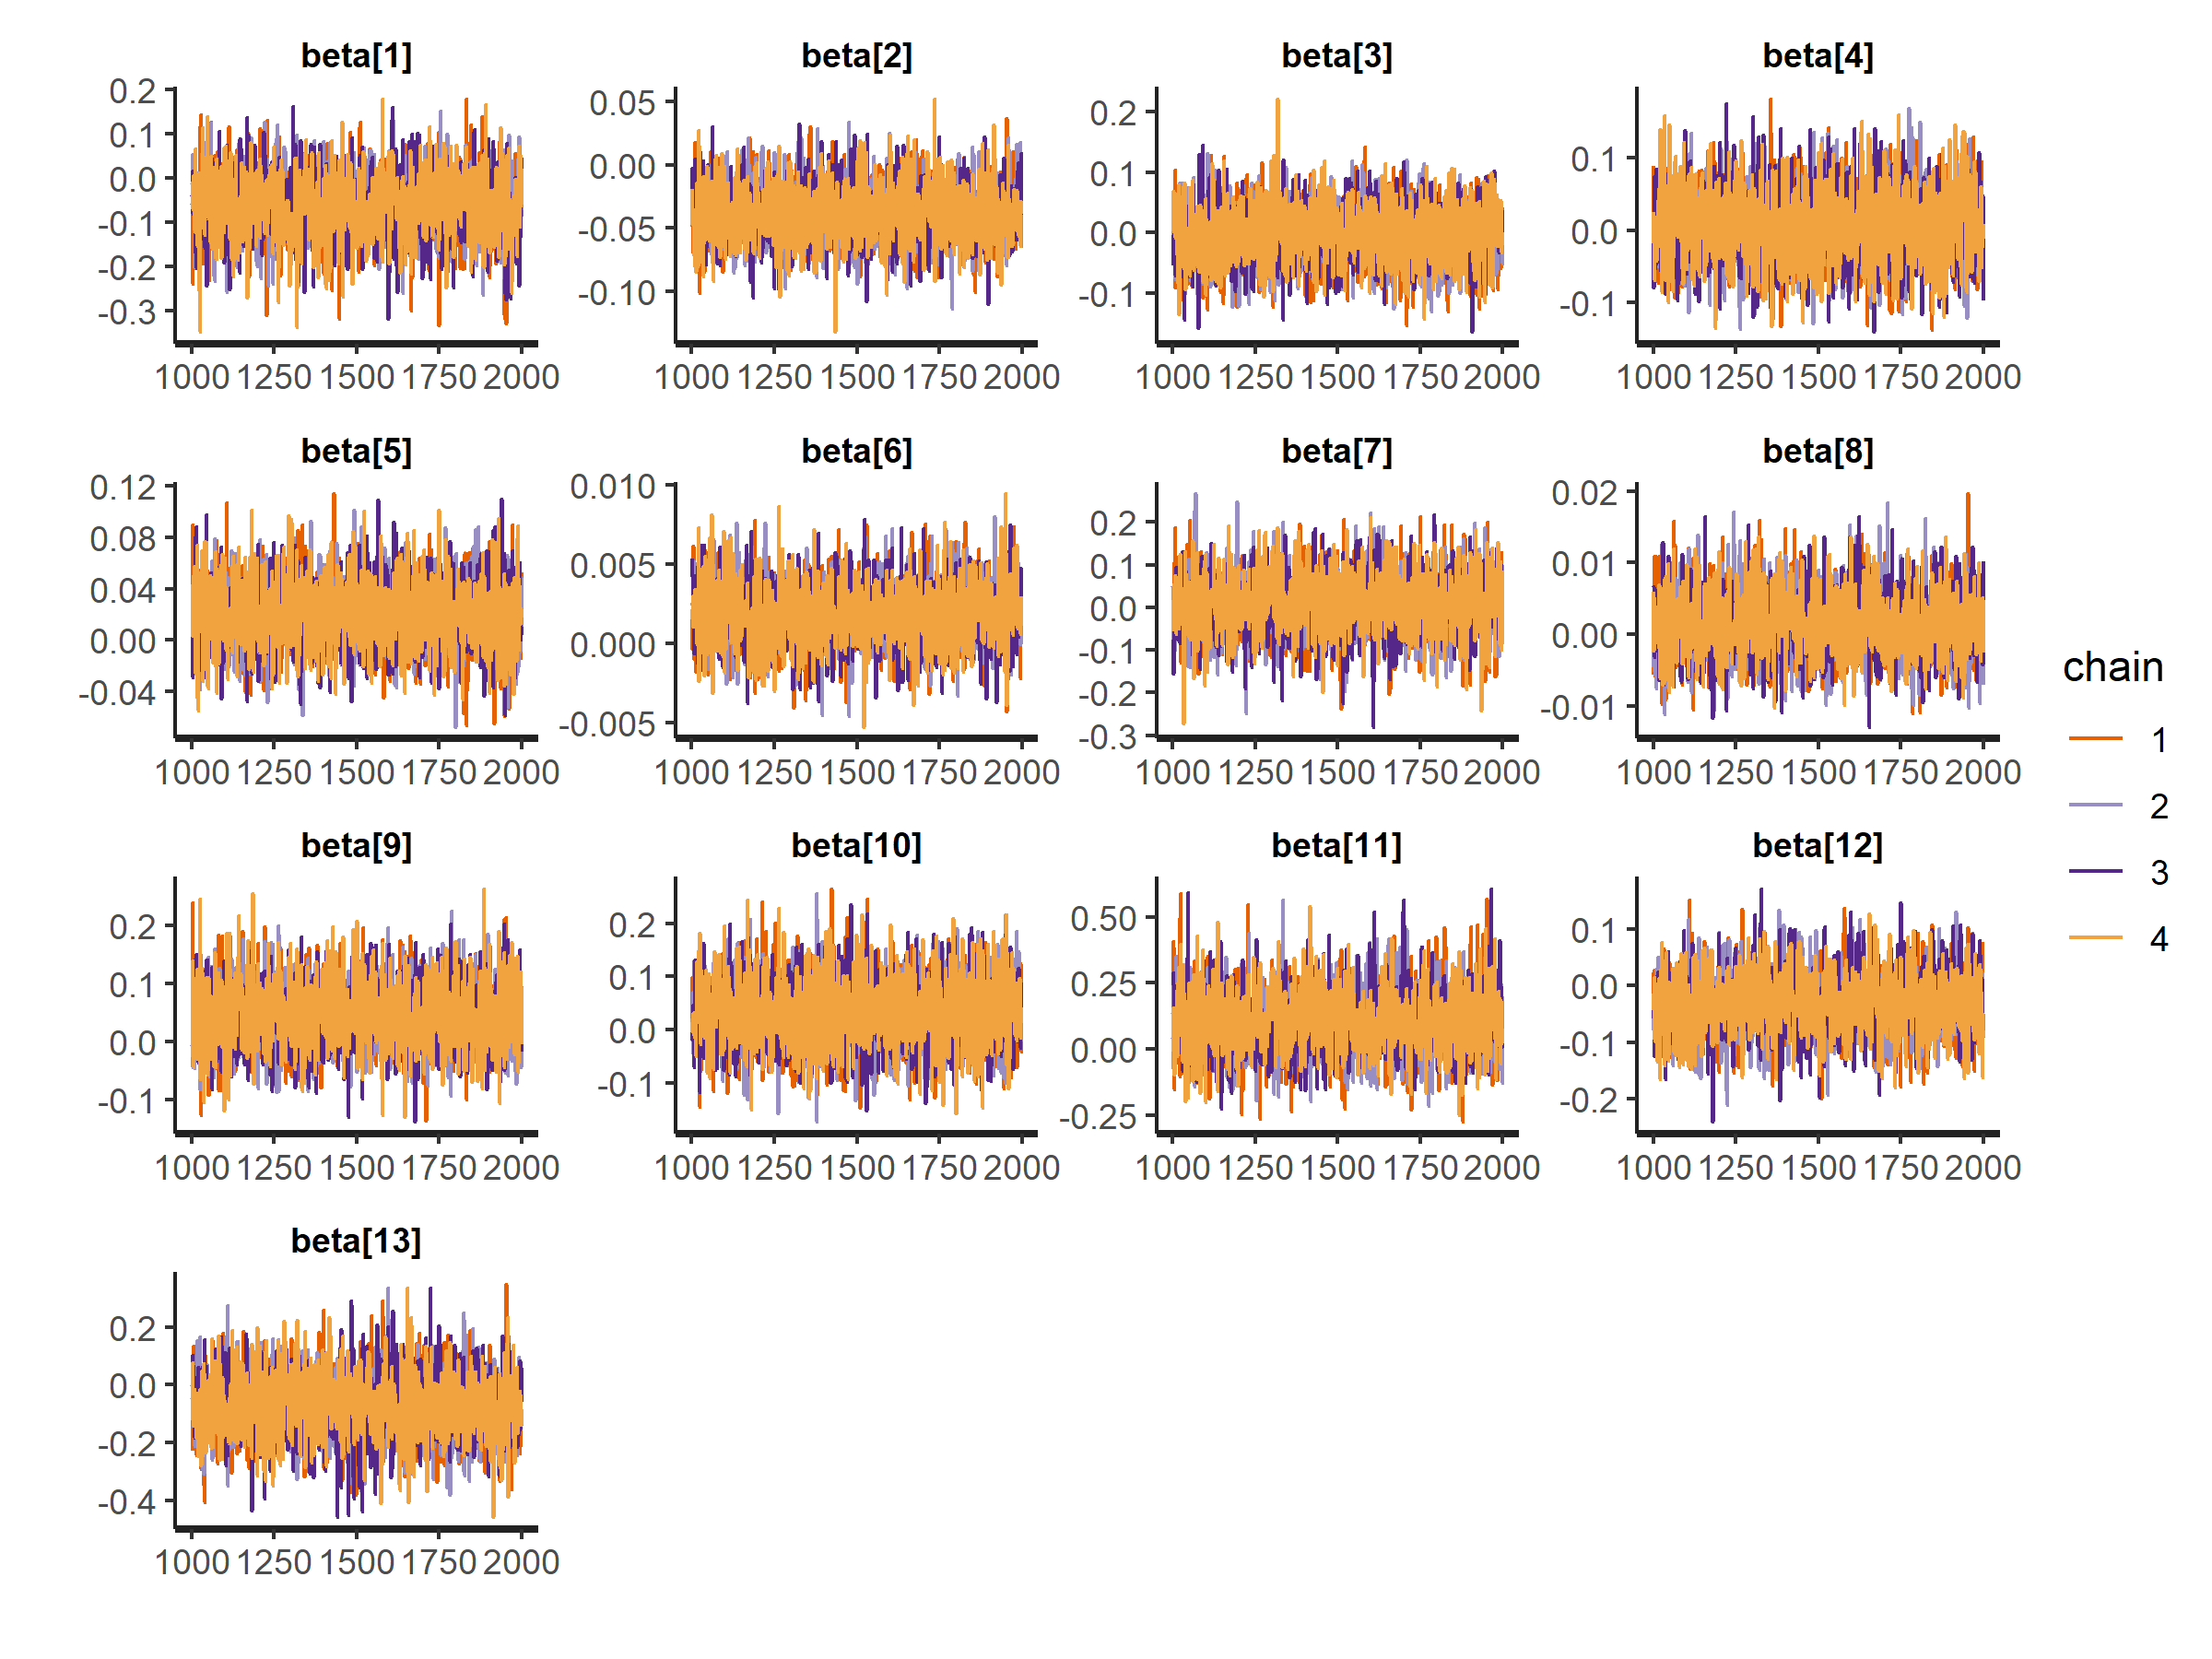
\includegraphics[width=0.95\textwidth]{trace-all-min.png}
	\caption{Traceplot of alliance level parameters in the non-major power sample.}
	\label{fig:trace-all-min}
\end{figure}



\section*{Normalizing Allied Capability}

% Justify use of annual normalization
As noted in the paper, I place allied capability in the membership matrix \textbf{Z} on the same scale as the other parameters by normalizing it by year. 
Within each year, I divide the total military spending of allied states by the maximum value, so capability values within each year range from just above zero to one. 
This ensures that allied capability is comparable within years, and that I do not treat more modern alliances as the most capable as raw defense budget sizes increase. 


The choice of this specific normalization is less theoretically informed than using capability itself. 
Therefore, I assessed the use of different normalizations and rescalings for allied capability by comparing model fit. 
I fit three models in addition to the one presented in the paper. 
The first rescaled allied capability by dividing each capability value by the maximum of capability without grouping alliances by year. 
The second rescaled alliance capability by dividing by two standard deviations, which is problematic because it introduces negative capability values. 
The last used total allied CINC scores instead of military spending as an indicator of allied capability, which also facilitates comparisons of allied capability within years. 
CINC scores measure the share of total world military capability each state has in a particular year, so it is useful for comparing allied capability within years \citep{SingerCINC1988}. 


After estimating these three models, I used leave-one-out (LOO) cross validation to assess model fit \citep{Vehtarietal2017}. 
LOO estimates pointwise out-of-sample prediction accuracy using the log-likelihood evaluated at the posterior simulations of the parameter values.\footnote{The widely applicable information criteria (WAIC) produces similar results, but the estimates for the CINC model may be driven by an unusual observation.} 
All diagnostics indicate the LOO results are not driven by unusual observations. 
As with other information criteria, lower values indicate better fit. 

 

\begin{table}[ht]
\centering
\begin{tabular}{rrrrrrrrr}
  \hline
 Allied Capability & elpd\_diff & se\_diff & elpd\_loo & se\_elpd\_loo  \\ 
  \hline
  Normalized by Year & 0.000 & 0.000 & -1159.513 & 184.714 \\ 
  Rescaled by Maximum & -3.165 & 2.643 & -1162.679 & 184.723  \\ 
  Recaled by 2SD & -10.749 & 6.116 & -1170.262 & 184.741  \\ 
  Total Allied CINC & -12.308 & 5.576 & -1171.821 & 184.683  \\ 
   \hline
\end{tabular}
\caption{Leave-one-out cross validation to assess model fit with different rescalings or normalizations of alliance capability. }
\label{tab:loo-zcontents}
\end{table}

\autoref{tab:loo-zcontents} summarizes the assessment of each model using the expected log pointwise predictive density (elpd). 
I use the model from the paper as the comparison model: a negative elpd\_diff implies the normalized model fits the data better. 
The difference also has some uncertainty, which is summarized by the se\_diff column of \autoref{tab:loo-zcontents}. 
The other three models have a negative elpd\_diff compared to the model with normalized capability by year. 
For the models with CINC and rescaling by two standard deviations the difference is large, relative to the se\_diff, so there is a clear preference for the normalized model. 
Normalizing by year provides at best a marginal improvement over a model where capability is rescaled using the maximum. 
Rescaling capability by the maximum produces similar inferences about alliance characteristics, including treaty depth. 



\section*{Fake Data Simulation Check}


With any complicated model, simulating fake data and seeing if the model can recover known parameters is essential. 
Fake-data simulation helps validate results from observed data and catch potential pathologies. 
This section summarizes results from fitting the multilevel model to fake data.


I simulated a dataset of 2000 t-distributed observations with 50 states observed for 200 years and 100 alliances. 
The outcome has a different scale than the military spending outcome variable, so coefficient values here do not match reported values in the paper.  
I then simulated two state and alliance level variables and a sparse matrix of state membership in alliances. 
Last, I ran the model without evaluating the likelihood, generating a posterior prediction of the outcome based on the fake data.


To check whether the model could recover known parameters, I took the 12th draw of the posterior distribution.
This draw included a simulated outcome for each observation and a set of coefficients. 
I then fit the multilevel model on the simulated outcome values and checked whether the credible intervals contained the corresponding parameter values. 
If a parameter is within the 90\% credible interval, the model captures it. 


The model recovers known parameters with a high degree of accuracy. 
As shown by \autoref{fig:beta-sim-res}, the two credible intervals of the alliance-level regression include the known values.
Credible interval coverage for the variance hyperparameters and $\gamma$ parameters is also acceptable. 


\begin{figure}[htbp]
	\centering
		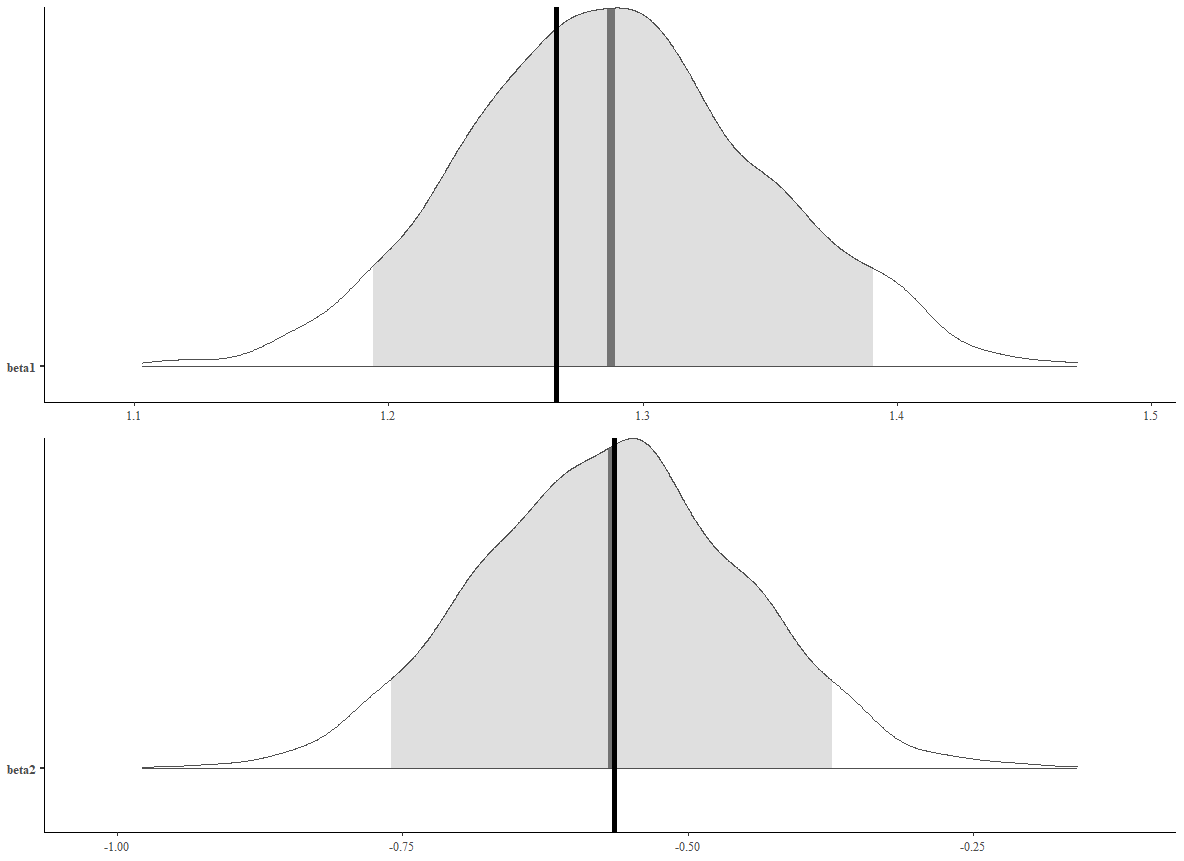
\includegraphics[width=0.95\textwidth]{beta-sim-res.png}
	\caption{Posterior distributions of $\beta$ parameters from fitting multilevel model to fake data. The black vertical line marks the known parameter value, and the grey area is the 90\% credible interval.}
	\label{fig:beta-sim-res}
\end{figure}


 
Even with small multiples, the 100 $\lambda$ parameters are harder to plot, so I offer a descriptive summary here. 
Among the $\lambda$ parameters, 93 of 100 intervals contain the known $\lambda$ value.
Given the large number of parameters and smaller sample, this is acceptable accuracy. 
Even the seven inaccurate confidence intervals were quite close--- all were within .015 of the known parameter.\footnote{Fine margins around these intervals implies that the exact number of accurate $\lambda$ intervals is sensitive to simulation variance.}


In summary, convergence diagnostics and fake data fitting both suggest that the multilevel model is working well. 
No convergence diagnostics indicate problems exploring the posterior. 
Just as importantly, the model can recover known parameters from fake data. 
The next section provides more detail on results from the major and non-major power samples. 




\section*{Robustness Check 1: Alternative Measure of Military Spending}

The main findings in the manuscript rely on the Correlates of War military spending. 
Due to reporting issues, definition problems and measurement challenges, other measures of military spending could lead to different results. 
I check the robustness of my results by using \citet{Nordhausetal2012}'s measure of military spending, which combines data from the COW project and the Stockholm International Peace Research Institute (SIPRI). 
\citet{DigiuseppePoast2016} use this measure of military spending in their paper. 


I estimate the same multilevel model on this measure of military spending, which covers from 1949 to 2001. 
This model also checks whether how treaty depth modifies the impact of alliance participation on military spending changes after World War II.
Because the coefficient on a lagged dependent variable in this model is close to one, implying a probable lack of stationarity in levels, I use changes in military spending as the outcome of interest. 


\begin{figure}[htbp]
	\centering
		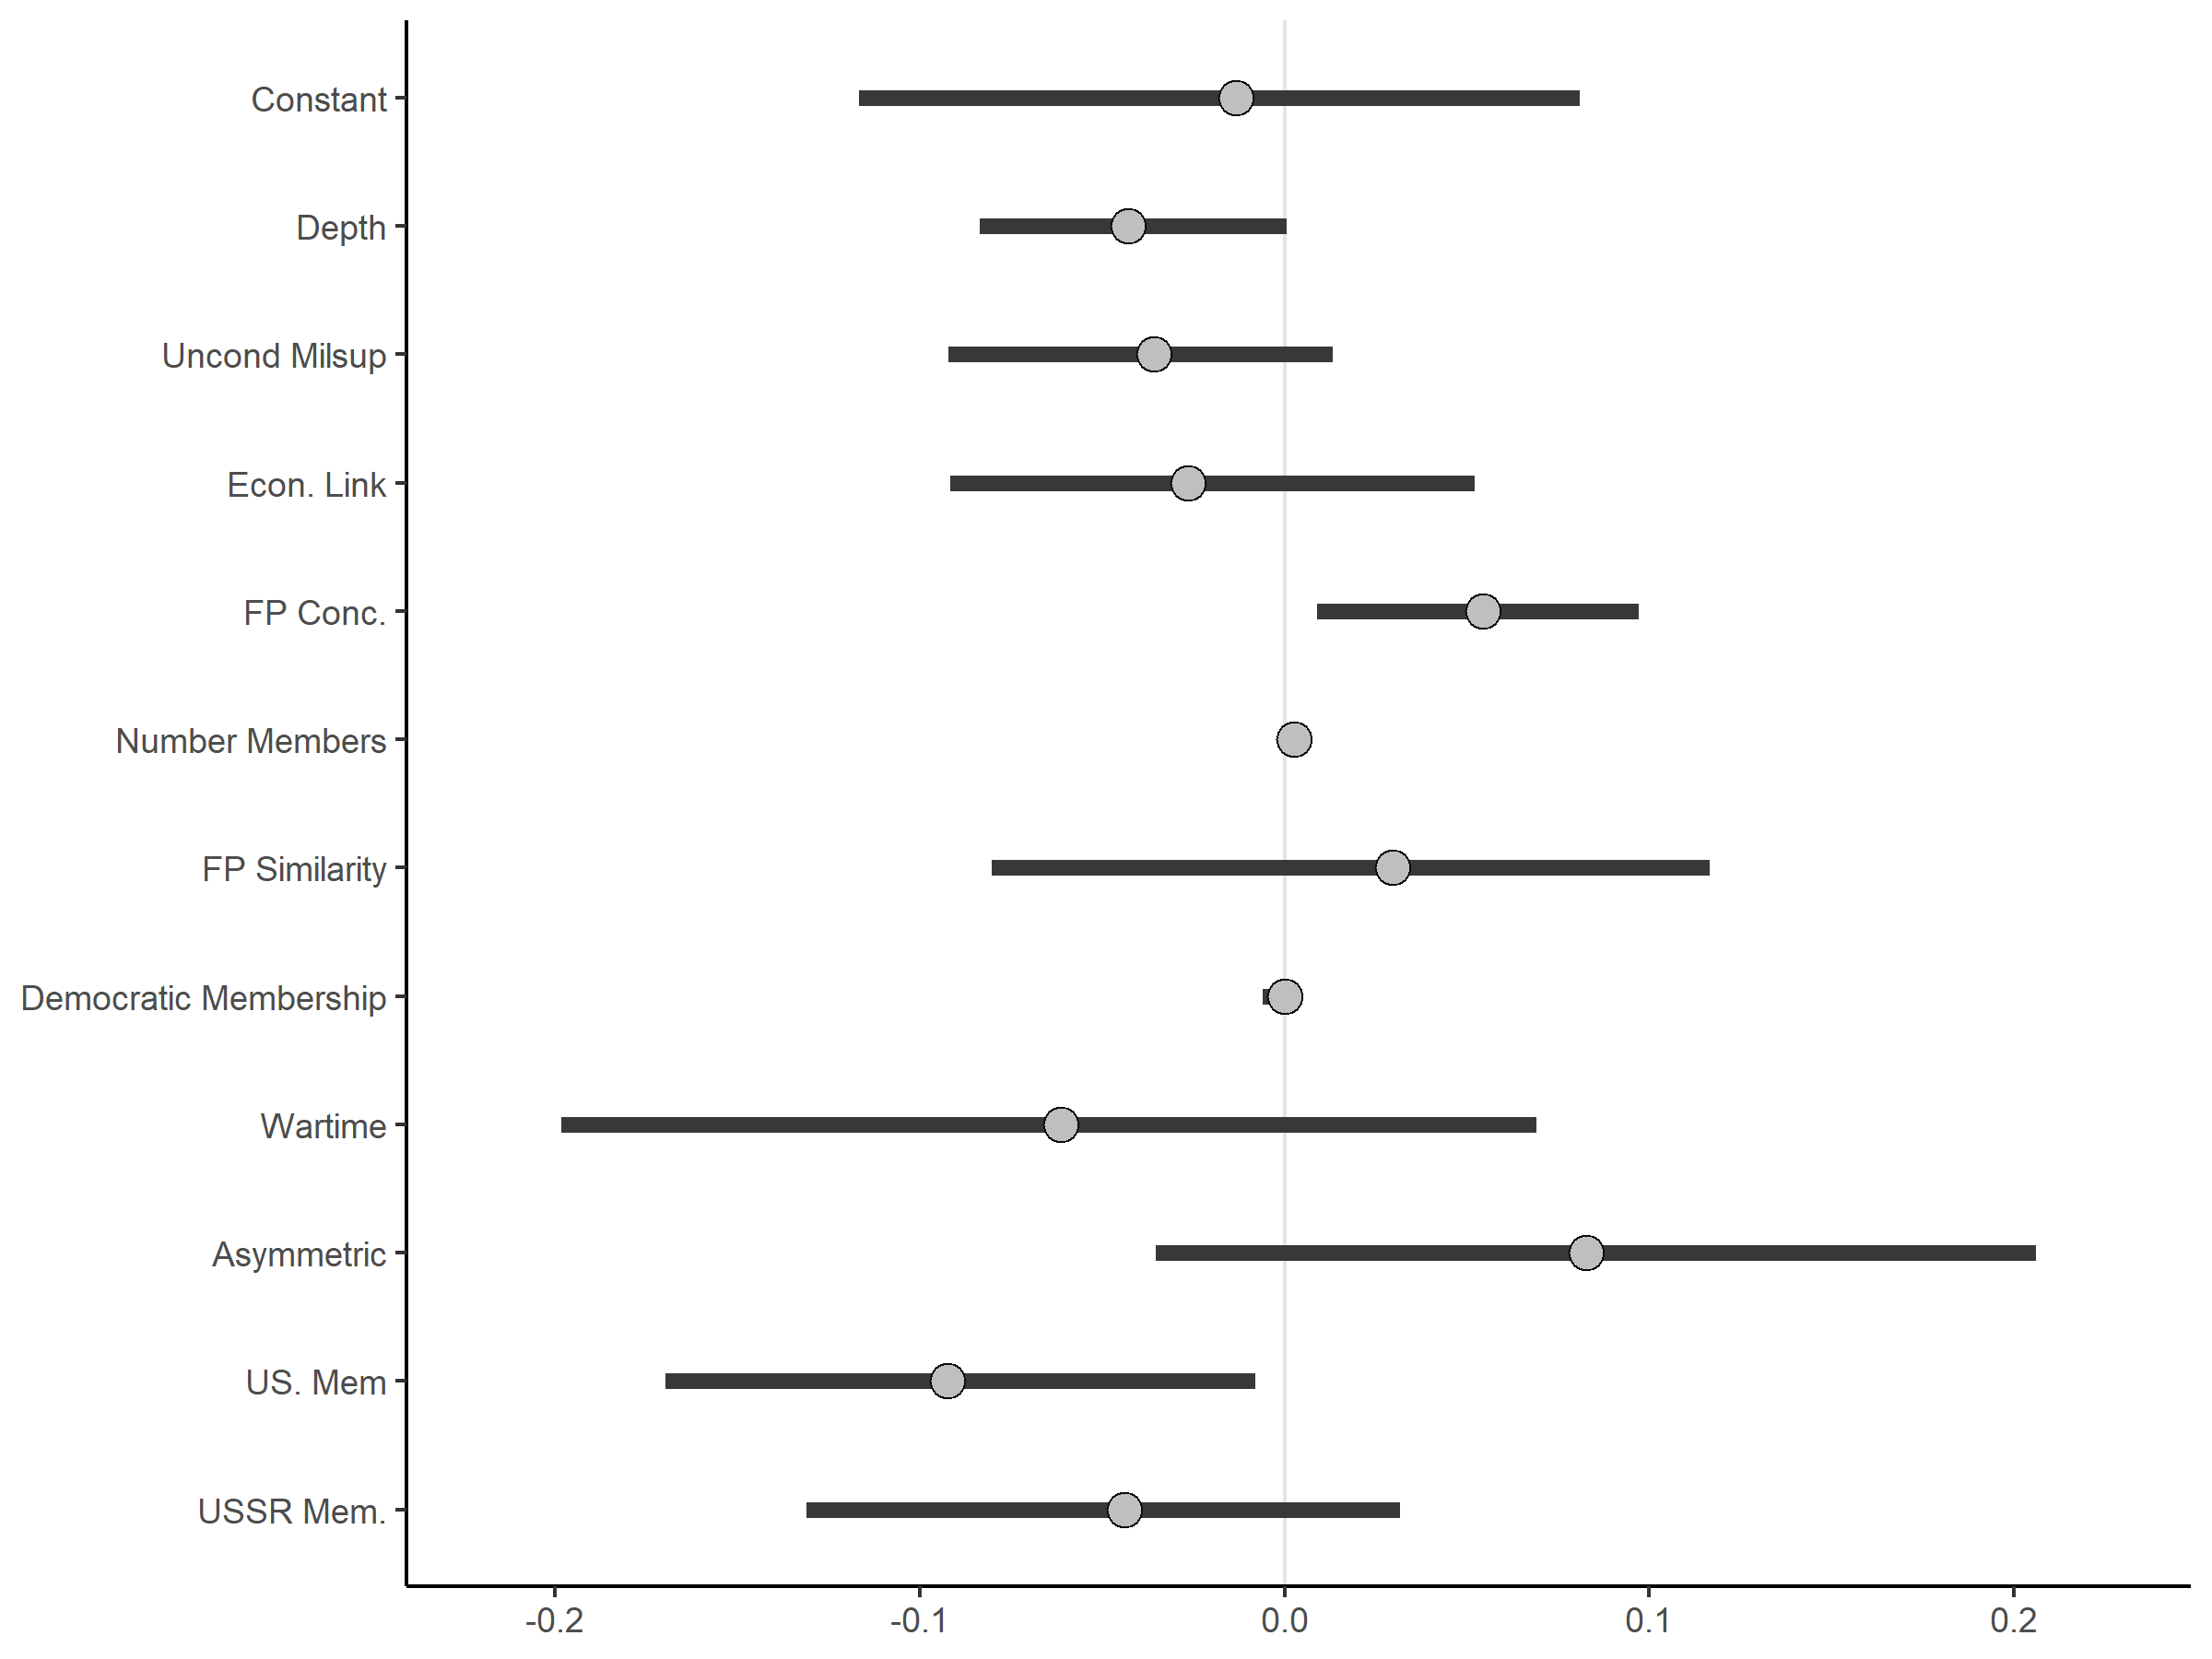
\includegraphics[width=0.95\textwidth]{post45-beta-res.png}
	\caption{90\% credible intervals of the $\beta$ parameters from an analysis of changes in non-major power military spending from 1949 to 2001.}
	\label{fig:post45-beta-res}
\end{figure}


\autoref{fig:post45-beta-res} summarizes the alliance-level regression parameters. 
As with the COW data, the credible interval for treaty depth is negative and does not overlap zero. 
All the parameter estimates are similar in this data, which increases my confidence that the results are not driven by the COW spending data. 

 


\section*{Robustness Check 2: Single-Level Regression}

Though the multilevel model best reflects the theory, I also fit some more standard panel data models. 
In what follows, I briefly present results from robust regressions of state-year percentage changes in military spending in the same sample of non-major powers. 
As in the multilevel model, I applied the inverse hyperbolic sine transformation to the outcome. 
In these models, I employ two indicators of alliance depth. 
The first is the average depth of a state's alliances. 
The second is a dummy which equals 1 if a state has at least one alliance with greater than average depth. 
Both variables compare states as the depth of their alliance portfolio shifts. 
In addition to the state-level controls in the multilevel model, I included averages of alliance size and democracy and the log of total allied capability as controls. 


I estimated several models, including robust regressions on all states, non-major powers, and non-major powers in alliances. 
I also applied fixed effects to an OLS model of percentage changes in defense expenditures. 
The estimated association between average treaty depth and military spending changes is summarized in \autoref{fig:single-level-mplot}. 
Results are inconsistent- the average depth measure fails to reject the null without fixed effects. 
The deep alliance dummy coefficient estimate is negative and statistically significant across several samples and model specifications, however. 

\begin{figure}[htbp]
	\centering
		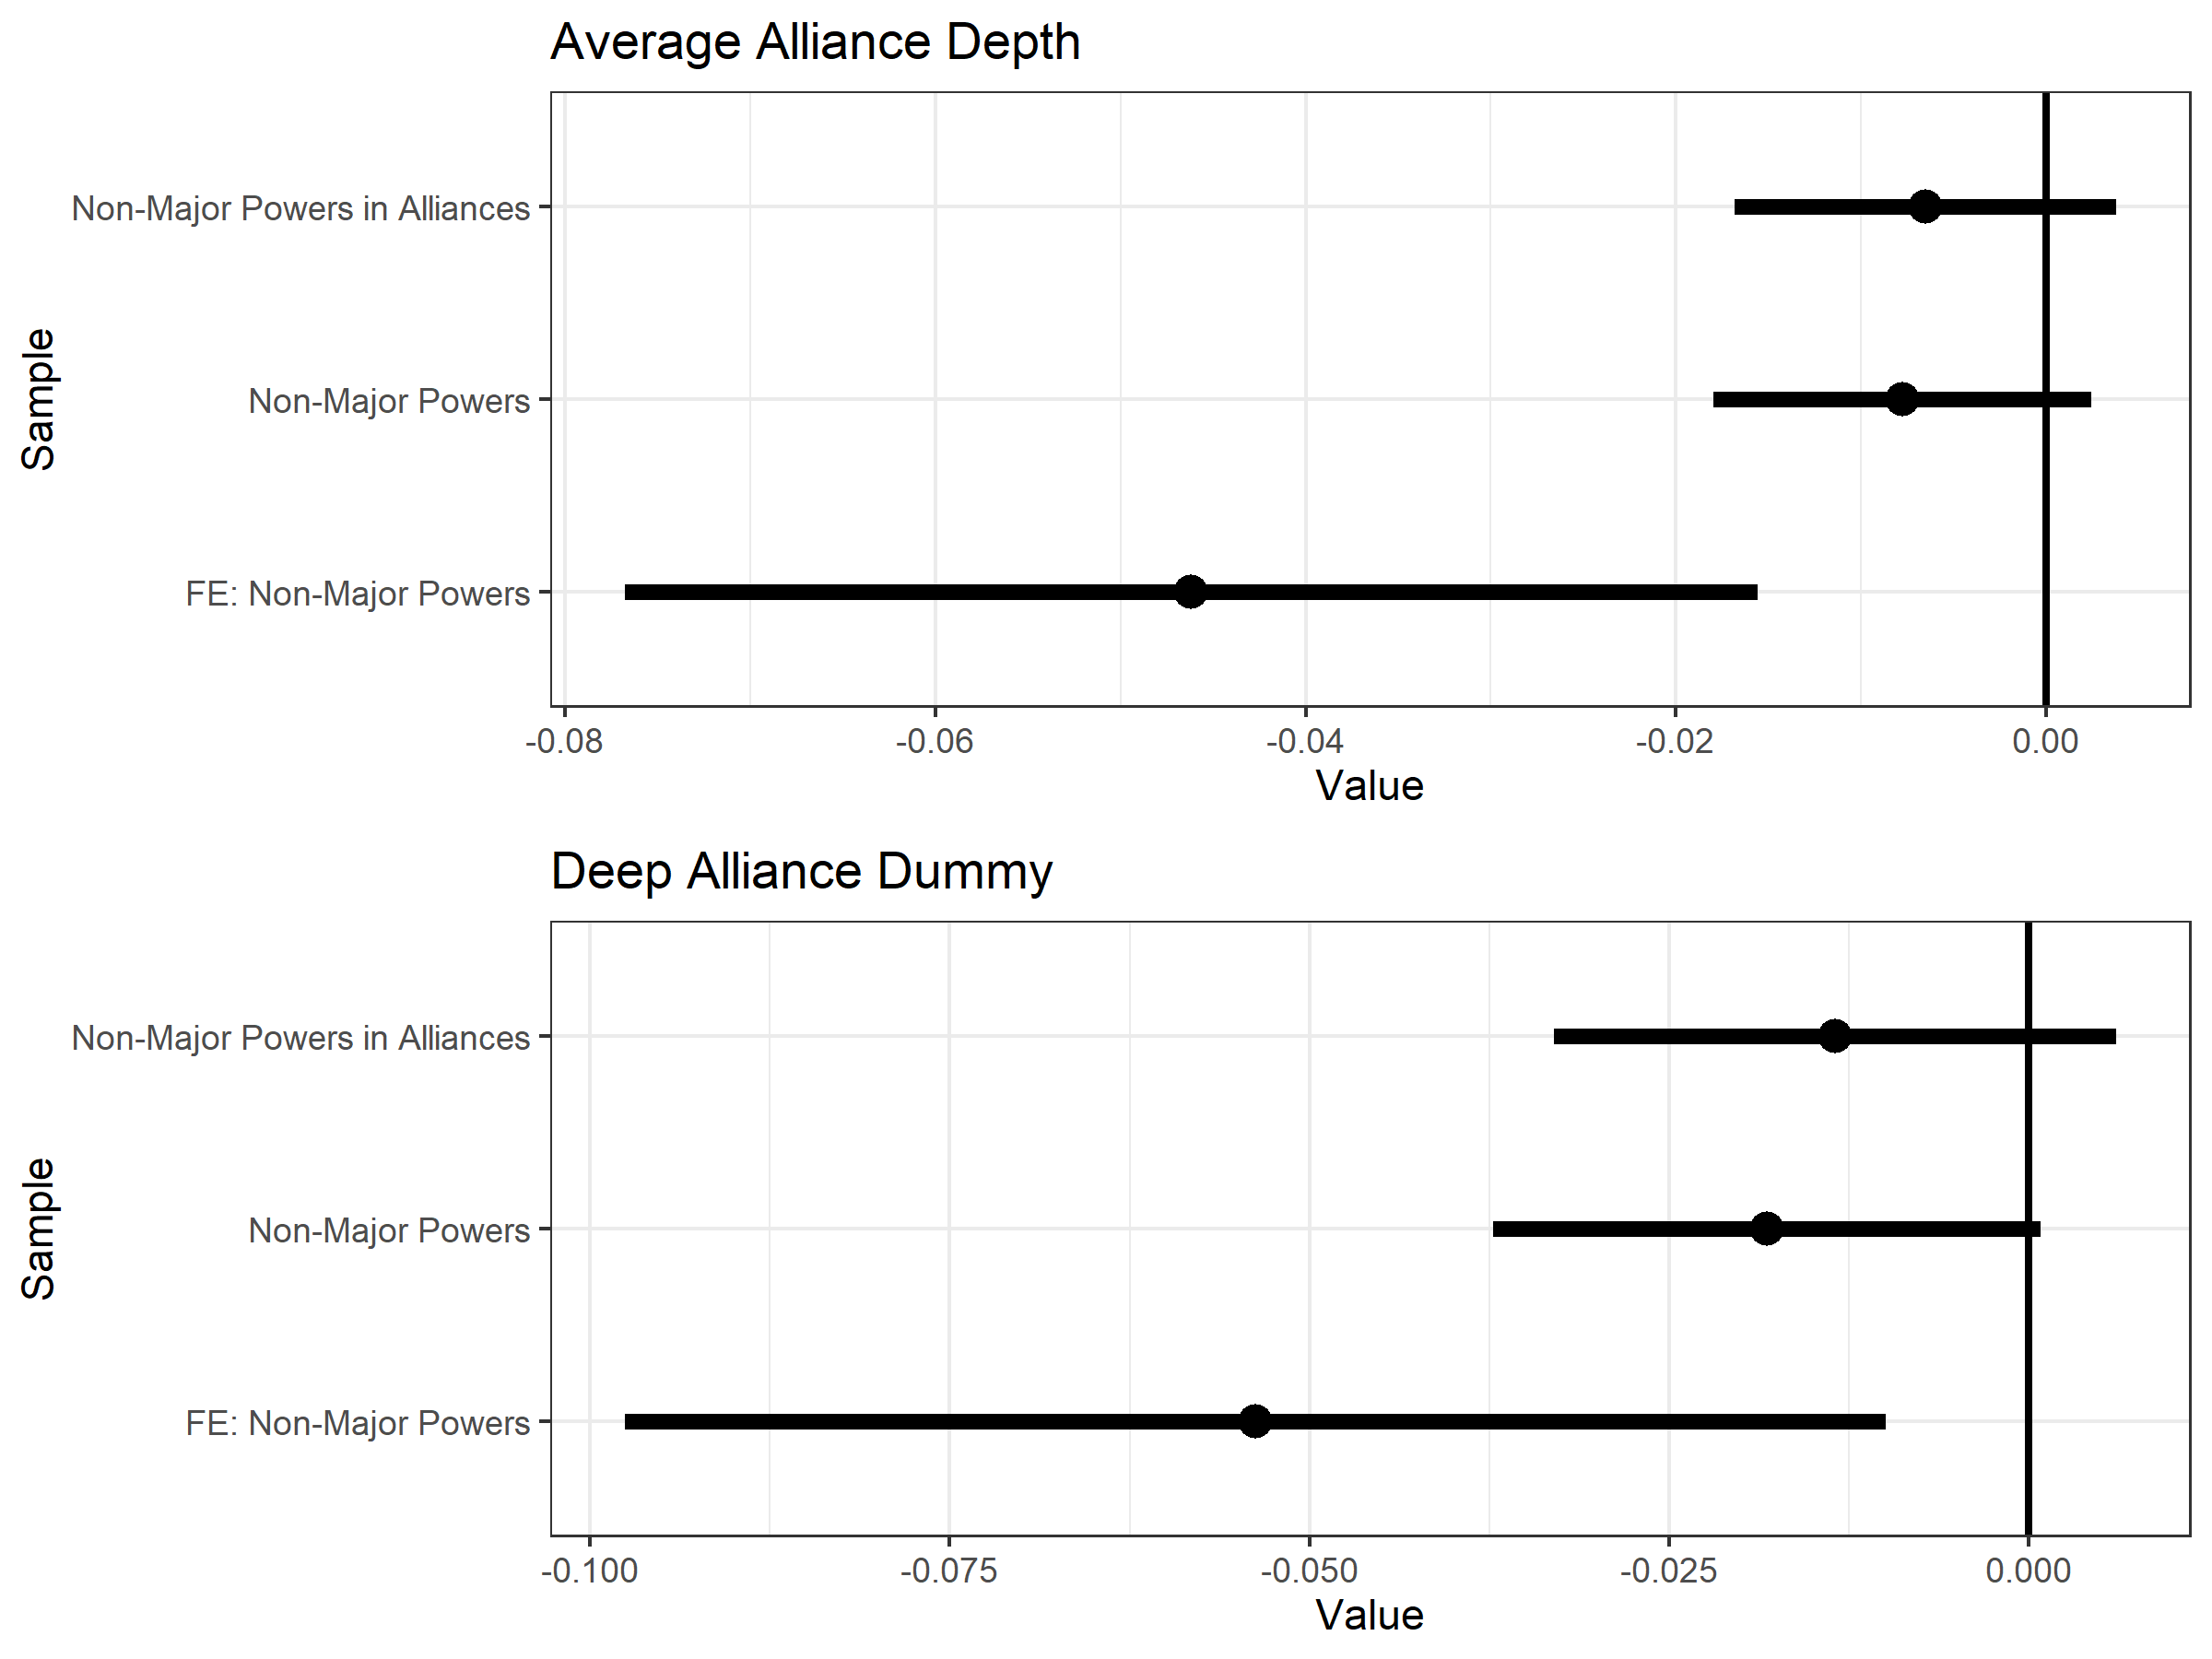
\includegraphics[width=0.95\textwidth]{single-level-mplot.png}
	\caption{Estimated effect of average alliance treaty depth or a dummy indicator of participation in a deep alliance on percentage changes in non-major power military spending.}
	\label{fig:single-level-mplot}
\end{figure}


The analysis of non-major powers in alliances is the best approximation of the multilevel model, as it compares non-major powers with different kinds of alliances. 
Analyzing a sample of all non-major powers includes states with no alliances, with does not match the comparison in the multilevel model. 
To assess the robustness of the coefficient estimate in the sample of non-major powers with alliances, I performed Extreme Bounds analysis. 
Specifically, I present results from \citet{Sala-i-Martin1997}'s method of bounds analysis in \autoref{fig:eba-single-level}. 


\autoref{fig:eba-single-level} shows the distribution of the deep alliance coefficient and an indicator of whether the alliance includes economic agreements. 
Across many specifications, where all regression coefficients are doubtful, the CDF of the deep alliance coefficient has 99\% negative mass. 
Even though the normality assumption is clearly violated, the histogram in \autoref{fig:eba-single-level} shows little evidence having a deep alliance increases percentage changes in military spending. 
The bounds analysis indicates a deep alliance dummy is a robust predictor of percentage changes in military spending across over 1500 single-level model specifications. 


\begin{figure}[htbp]
	\centering
		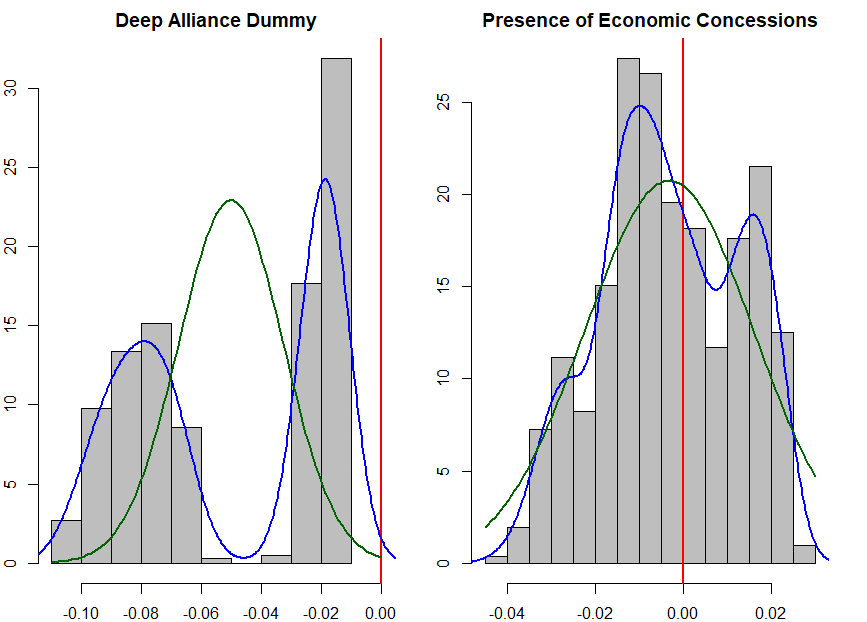
\includegraphics[width=0.95\textwidth]{eba-single-level.png}
	\caption{Histogram of coefficient values for a deep alliance dummy and economic concessions in at least one alliance in a single-level robust regression of non-major powers in alliances.}
	\label{fig:eba-single-level}
\end{figure}



  
\bibliography{../../MasterBibliography} 




\end{document}
